% ПРОЧИТАЙ МЕНЯ
% ПРОЧИТАЙ МЕНЯ
% ПРОЧИТАЙ МЕНЯ
%
% В этом файле вы описываете задачи из контеста
% Условия можно вставить в виде фотографий
% В идеях нужно написать хотя бы два-три предложения о задаче
% Если задача довольно трудная, описание идеи должно быть подробным
% Комментарии в исходном коде приветствуются
% Положение тоже можно фотографией
%
% ПРОЧИТАЙ МЕНЯ
% ПРОЧИТАЙ МЕНЯ
% ПРОЧИТАЙ МЕНЯ

\includepdf[pages=10, scale=0.75, pagecommand={
\begin{center}
\bfseries{\large ТЕХНИЧЕСКИЙ ОТЧЁТ ПО ПРАКТИКЕ}
\end{center}
\subsection*{Grand Prix of Dolgoprudny 12.09.2021}
}]{statements/210912/210830.pdf}
\subsubsection*{Идея решения}
Очевидно, что нужно всегда брать грани монет, которые присутствуют у оппонентов, то есть при наличии только одной монеты со значениями $1$ и $2$ не имеет смысла брать номинал $3$ на одну из граней нашей монеты, так как можно взять $2$ и потратить меньше денег. Пока мы не взяли ни одной грани полагаем, что наше математическое ожидание равняется $bad = -\sum_{i}x_i$, пусть тогда мы взяли на одну из сторон монеты $a'$, а на другую $b'$, тогда наше математическое ожидание равняется $E(a',b') = \sum_{i : a_i \leqslant a'}(\frac{x_i}{2}) + \sum_{i : b_i \leqslant a'}(\frac{x_i}{2}) + \sum_{i : a_i \leqslant b'}(\frac{x_i}{2}) + \sum_{i : b_i \leqslant b'}(\frac{x_i}{2}) + bad - a' \cdot b'$. Закинем все значения $a_i$ и $b_i$ в массив $z$ с коэффициентами $\frac{1}{2}$, отсортируем, посчитаем $pref_i = \sum_{j = 0}^{i - 1}z_i$. Упростим нашу сумму для подсчета математического ожидания: $E(a',b') = pref_{i'} + pref_{j'} + bad - a \cdot b$, где $i' : z_{i'} = a'$ и $j' : z_{j'} = b'$. В таком случае мы можем посчитать ответ за $O(n ^ 2 + n \cdot \log{n}) \approx O(n ^ 2)$ перебрав индексы в $z$. Улучшим решение до $O(n \cdot \log{n})$. Пусть мы уже выбрали $a'$, тогда мы хотим выбрать $b'$ такое, что $E(a', b') \rightarrow max$. Т.е. $E(a') = max_{b' \leqslant a'}(a'\cdot b' + pref_{j'}) + bad + pref_{i'}$. Заметим, что $a'\cdot b' + pref_{j'}$ при фиксированной $a'$ является прямой с $k = b'$ и $b = pref_{j'}$. В таком случае можно воспользоваться \textit{Convex hull trick}. Мы будем хранить множество прямых слева направо, так как угол наклона растет, то новую прямую мы будем добавлять справа, а также $a'$ тоже растет, поэтому мы сможем быстро узнавать максимум. Этот прием работает амортизованно за $O(n)$. Итоговая сложность: $O(n + n \cdot \log{n}) \approx O(n \cdot \log{n})$.
\subsubsection*{Исходный код}
\lstinputlisting{src/gp_dolgop_g.cpp}
\subsubsection*{Фрагмент турнирной таблицы}
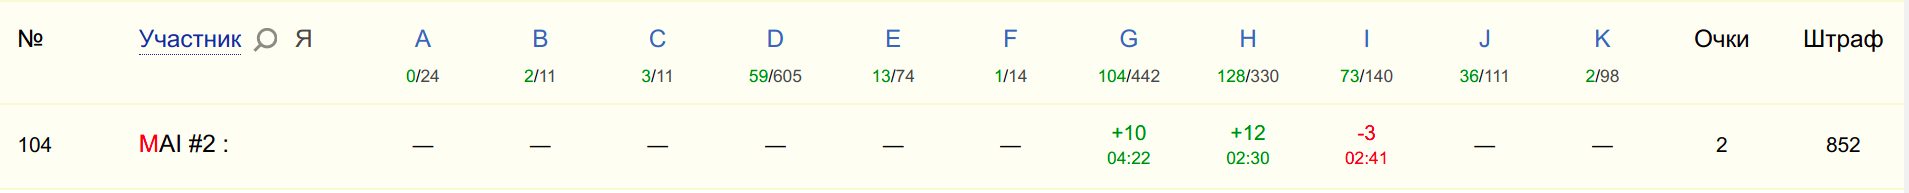
\includegraphics[width=\textwidth]{images/gp_dolgop.png}\newline\noindent
\subsubsection*{Выводы}
Задача решена. Было 10 неудачных попыток.
\pagebreak

\includepdf[pages={11}, scale=0.75, pagecommand=\subsection*{Grand Prix of IMO 19.09.2021}]{statements/210919/day3.en.pdf}
\subsubsection*{Идея решения}
Как известно, задача поиска Гамильтонова пути в графе является NP-полной. С помощью динамического программирования по подмножествам вычислительную сложность можно уменьшить с $O(n!)$ до $O(n ^ 2 \cdot 2 ^ n)$. Реализуем алгоритм, проверяющий какой-то граф на наличие Гамильтоновых путей между $K$ парами вершин $u$ и $v$.

Для маленьких $K$ нетрудно найти ответ. Для большего $K$ будем случайно генерировать графы и искать в них количество пар вершин $u$ и $v$ таких, что между ними есть Гамильтонов путь. Сгенерировав достаточно графов, можно увидеть закономерность, тогда решение становится полностью конструктивным, его асимптотика $O(K)$.

\subsubsection*{Исходный код}
\lstinputlisting{src/gp_imo_h.cpp}
\subsubsection*{Фрагмент турнирной таблицы}
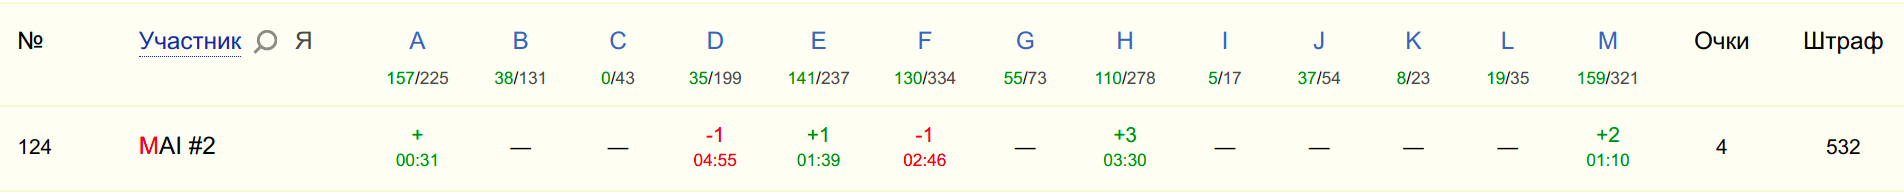
\includegraphics[width=\textwidth]{images/gp_imo.png}\newline\noindent
\subsubsection*{Выводы}
Задача решена. Было 3 неудачных попытки.
\pagebreak

\includepdf[pages={2, 3}, scale=0.75, pagecommand=\subsection*{XXII Открытая Всесибирская олимпиада 10.10.2021}]{statements/211010/sib.pdf}
\subsubsection*{Идея решения}
Для решения задачи требуется аккуратно реализовать проверку условий уровней конфликта. Если найденные моменты времени не противоречат условиям, то ответ <<Freytag>>, иначе <<Nein>>. Сложность решения $O(n)$.

\subsubsection*{Исходный код}
\lstinputlisting{src/sib_a.cpp}
\subsubsection*{Фрагмент турнирной таблицы}
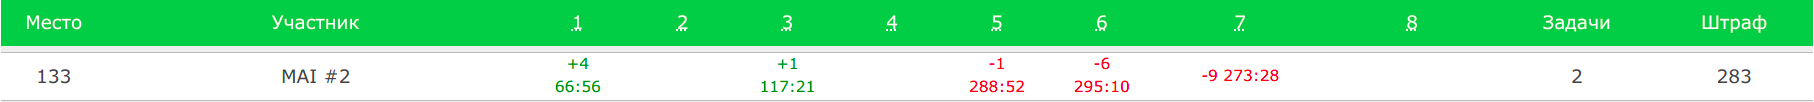
\includegraphics[width=\textwidth]{images/sib.png}\newline\noindent
\subsubsection*{Выводы}
Задача решена. Было 4 неудачных попытки.
\pagebreak

\includepdf[pages={8, 9}, scale=0.75, pagecommand=\subsection*{ICPC training MAI 21-22 17.10.2021}]{statements/211017/training1mai21.pdf}
\subsubsection*{Идея решения}
Для проверки подлинности таблицы составим наихудший и наилучший возможный рейтинг команды. Зная это, мы можем легко проверить, является ли часть таблицы верной. Асимптотика решения $O(n \cdot (k + m))$.

\subsubsection*{Исходный код}
\lstinputlisting{src/training1mai21_f.cpp}
\subsubsection*{Фрагмент турнирной таблицы}
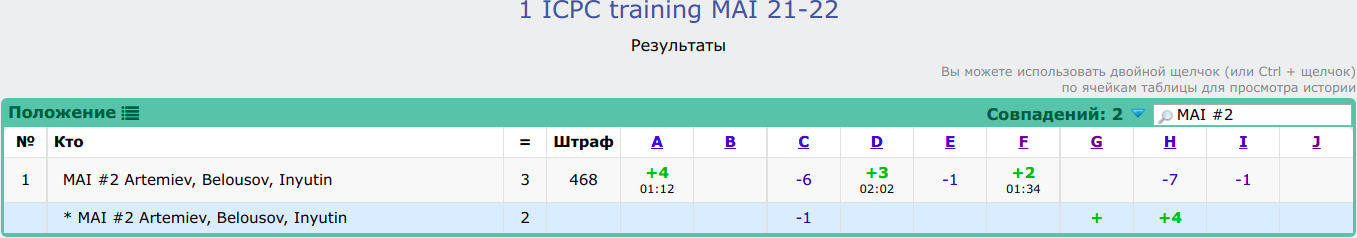
\includegraphics[width=\textwidth]{images/training1mai21.png}\newline\noindent
\subsubsection*{Выводы}
Задача решена. Было 2 неудачных попытки.
\pagebreak

\includepdf[pages={12}, scale=0.75, pagecommand=\subsection*{Grand Prix of Korea 24.10.2021}]{statements/211024/contest-24341-en.pdf}
\subsubsection*{Идея решения}
Давайте решим задачу для одного бита. Понятно, что решив такую задачу мы сможем с легкостью решить изначальную задачу ввиду того, что \textit{OR} одного бита не влияет на остальные.

Построим граф, вершины будут представлять собой регистры. Добавим ориентрированные ребра, ребро из $a$ в $b$ с весом $w$ будет обозначать, что $w$ команда будет присваивать $x_b = x_b | x_a$. Тогда нам потребуется найти минимальное время для каждой вершины, через которое произойдет замена бита $0$ на $1$. Это проблема легко решается с помощью алгоритма Дейкстры: просто запустим Дейкстру из всех таких регистров, в которых изначально стоит $1$, и немного поменяем метрику при пересчете расстояний.

Проделаем данный алгоритм для всех $8$ битов. В конце концов, для каждой вершины поставим $1$ в $i$-ом бите, если мы успеем его достичь быстрее чем за $t$ операций.

Итого решение работает за такую асимптотику $O(k \cdot l \cdot \log{n})$, где $k$ - это количество битов, в нашем случае $k = 8$.

\subsubsection*{Исходный код}
\lstinputlisting{src/gp_korea_j.cpp}
\subsubsection*{Фрагмент турнирной таблицы}
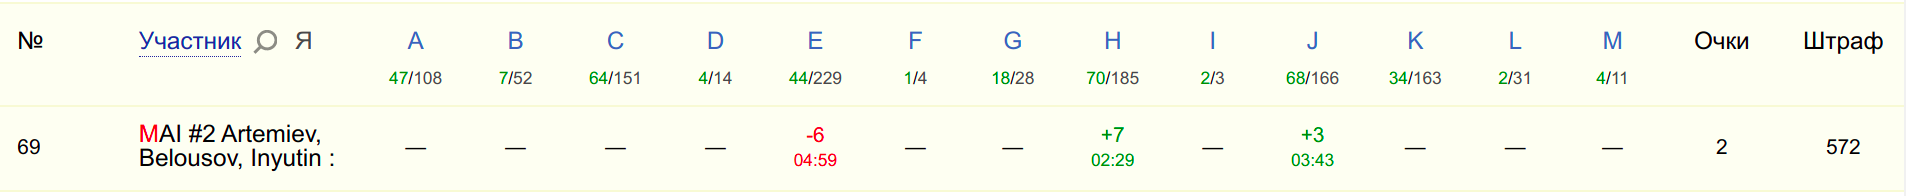
\includegraphics[width=\textwidth]{images/gp_korea.png}\newline\noindent
\subsubsection*{Выводы}
Задача решена. Было 7 неудачных попыток.
\pagebreak

\includepdf[pages={5, 6}, scale=0.75, pagecommand=\subsection*{Grand Prix of Siberia 07.11.2021}]{statements/211107/ocmgp5.ru.pdf}
\subsubsection*{Идея решения}
Основная сложность --- правильно реализовать систему штрафов в хоккее. Для этого каждую секунду игры. Если в какой-то момент времени на поле произошло событие, то его следует обработать согласно правилам игры. Для этого для каждого игрока обеих команд будем хранить тип штрафа и оставшееся время вне игры, постепенно уменьшая его. Остаётся проверять, сколько игроков на поле и увеличивать время для соответствующего состояния игры. Моделирование работает за константу, поэтому сложность решения $O(60 \cdot 60 \cdot 10 + n) \approx O(n)$.

\subsubsection*{Исходный код}
\lstinputlisting{src/gp_siberia_5.cpp}
\subsubsection*{Фрагмент турнирной таблицы}
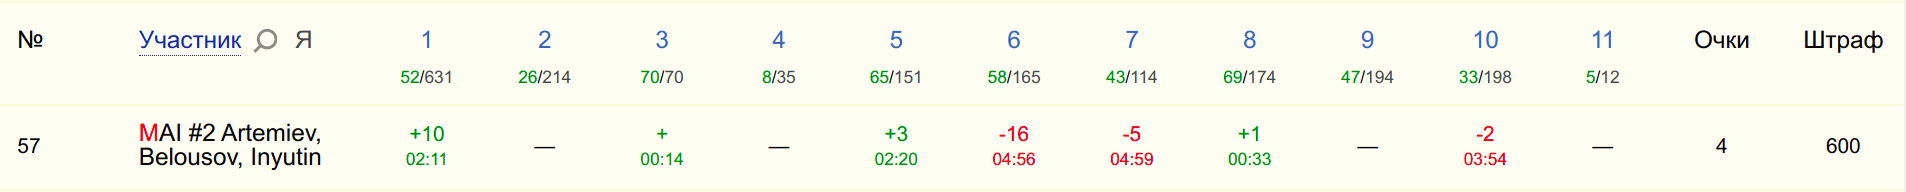
\includegraphics[width=\textwidth]{images/gp_siberia.png}\newline\noindent
\subsubsection*{Выводы}
Задача решена. Было 3 неудачных попытки.
\pagebreak

\includepdf[pages=3, scale=0.75, pagecommand=\subsection*{Grand Prix of EDG 14.11.2021}]{statements/211114/ocmgp6.en.pdf}
\subsubsection*{Идея решения}
Тривиальный случай, когда изменяется только одна цифра суммы, нам не очень интересен, так как изменяется всего две цифры во всех числах. Гораздо более сложный случай --- замена девяток на нули и нулей на девятки при изменении суммы. Заметим, что для какого-то префикса числа достаточно знать количество цифр <<0>> и <<9>>, чтобы корректно отвечать на запрос.

Используем струкуру данных, поддерживающую модификацию на отрезке для эффективного ответа на запрос и изменение. Во время контеста было реализовано решение с использованием Декартова дерева, которое не прошло по времени из-за большой константы. При дорешивании было реализовано решение, использующее дерево отрезков.

Сложность операций с деревом $O(\log{n})$. Асимптотика решения $O(n \cdot \log{n} + q \cdot \log{n})$.

\subsubsection*{Исходный код}
\lstinputlisting{src/gp_edg_b.cpp}
\subsubsection*{Фрагмент турнирной таблицы}
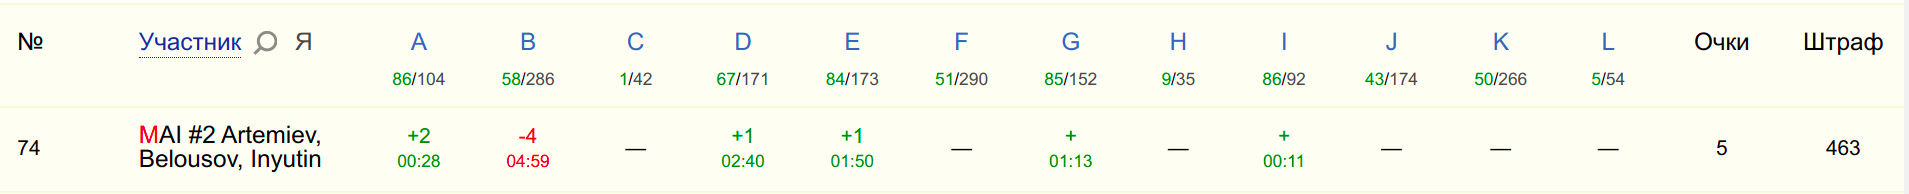
\includegraphics[width=\textwidth]{images/gp_edg.png}\newline\noindent
\subsubsection*{Выводы}
Задача дорешена.
\pagebreak

\includepdf[pages=2, scale=0.75, pagecommand=\subsection*{RuCode 4.0 Div A-B Champoinship 21.11.2021}]{statements/211121/rucodeAB-ru.pdf}
\subsubsection*{Идея решения}
Решение задачи полностью конструктивное, полностью описано в программе. Самый сложный случай --- при нечётных ширине или высоте складов СберМаркета. Асимптотика $O(w \cdot h)$.
\subsubsection*{Исходный код}
\lstinputlisting{src/rucode_b.cpp}
\subsubsection*{Фрагмент турнирной таблицы}
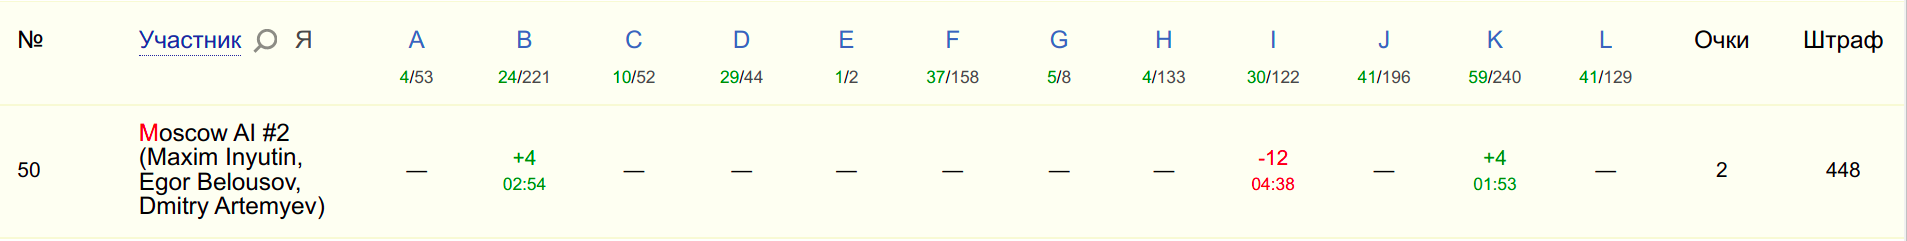
\includegraphics[width=\textwidth]{images/rucode.png}\newline\noindent
\subsubsection*{Выводы}
Задача решена. Было 4 неудачных попытки.
\pagebreak

\includepdf[pages={14,15}, scale=0.75, pagecommand=\subsection*{Div A + B Contest 1 22.11.2021}]{statements/211122/211122.en.pdf}
\subsubsection*{Идея решения}
Для решения задачи построим дерево отрезков на сумму чисел, стоящих на чётных и нечётных позициях для всего забора. Будет обновлять каждый фрагмент забора и выводить требуемую сумму. Так как суммарно обновлений в дереве будет не более $\sum a_i \leqslant 10 ^ 6$ и $n \leqslant 10 ^ 6$, то итоговая временная сложность решения $O(n \cdot \log{n})$.
\subsubsection*{Исходный код}
\lstinputlisting{src/mw1_f.cpp}
\subsubsection*{Фрагмент турнирной таблицы}
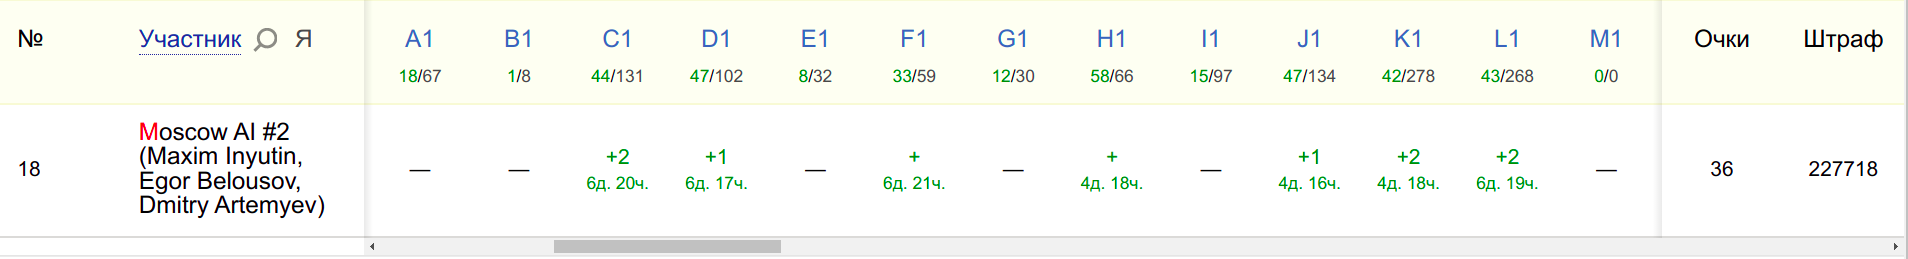
\includegraphics[width=\textwidth]{images/mw1.png}\newline\noindent
\subsubsection*{Выводы}
Задача дорешена.
\pagebreak

\includepdf[pages=21, scale=0.75, pagecommand=\subsection*{Div A Contest 4: The Korean Contest 26.11.2021}]{statements/211126/211126.en.pdf}
\subsubsection*{Идея решения}
Используем \textit{std::bitset} для эффективного хранения чисел. Для каждого разряда и для каждой цифры хранится битовое множество позиций чисел из множества $A$. Добавление и удаление чисел из такой структуры очень простое и выполняется фактически за $O(1)$. Пространственная сложность такого хранения $O({{4 \cdot 9 \cdot n}\over{64}}) \approx O(n)$.

Зафиксируем два числа тройки. Выберем только те цифры, которые удовлетворяют условию тройки, добавим в ответ количество индексов чисел. Операция \textit{count} для \textit{std::bitset} выполняется за $O({n \over 64})$, поэтому временная сложность решения $O({{n ^ 3} \over 64})$.
\subsubsection*{Исходный код}
\lstinputlisting{src/mw4_l.cpp}
\subsubsection*{Фрагмент турнирной таблицы}
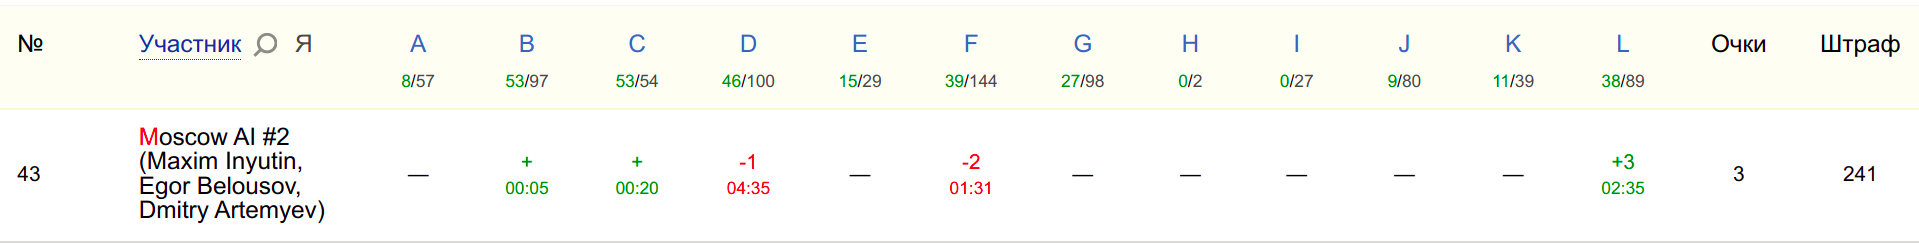
\includegraphics[width=\textwidth]{images/mw4.png}\newline\noindent
\subsubsection*{Выводы}
Задача решена. Было 3 неудачных попытки.
\pagebreak

% Можно и другую задачу
\includepdf[pages={14,15}, scale=0.75, pagecommand=\subsection*{Grand Prix of Nanjing 12.12.2021}]{statements/211212/ocmgp9.en.pdf}
\subsubsection*{Идея решения}
Решим сперва чуть более простую задачу, в которой бабочки улетают через 1 или 2 секунды. Возьмем вершину $1$ за корень дерева.
Пусть мы зашли в какую-то вершину и испугали всех смежных бабочек, тогда в вершины, где бабочки улетают через $1$ или $2$ секунды после испуга, мы, если хотим собрать бабочек, должны заходить сразу же, так как, если мы зайдем в другую вершину дерева, то нам придется потратить по крайней мере $3$ секунды.
Тогда пусть $dp_i$ обозначает максимальное кол-во бабочек, которые мы соберем, если начнем собирать в вершине $i$. Пересчет динамики таков: $dp_i = max_{j}\{\sum_{c \neq j}(dp_c - a_c) + dp_j\}$ где $j$ и $c$ являются детьми $i$ в дереве, с корнем в $1$.
Для того, чтобы пересчитать динамику в вершинах с $3$ секундами введем еще значение $dpvis_i$ --- сколько бабочек мы соберем, начиная с вершины $i$, если мы не возьмем бабочек в вершине $i$, а также во всех детях $i$, но возьмем бабочек во всех детях детей $i$. Пересчет достаточно прост: $dpvis_i$ = $\sum_{c}(dp[c] - a[c])$, где $c$ --- ребенок $i$. В конце концов пересчитаем динамику для $i$ дополнительно по вершинам с испугом в $3$ секунды: $dp_i = max_{j, k : j \neq k}\{\sum_{c \neq j, c \neq k}(dp_c - a_c) + dpvis_k + a_k + dp_j\}$, $j$ вершина с испугом в 3 секунды. Итого, используя поиск в глубину и предпосчитав суммы через префиксные суммы, можно решить данную задачу за $O(n)$
\subsubsection*{Исходный код}
\lstinputlisting{src/gp_nanjing_h.cpp}
\subsubsection*{Фрагмент турнирной таблицы}
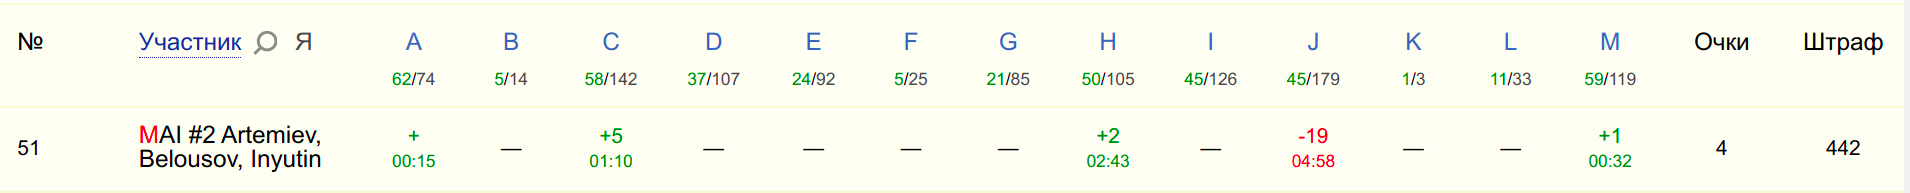
\includegraphics[width=\textwidth]{images/gp_nanjing.png}\newline\noindent
\subsubsection*{Выводы}
Задача решена. Было 2 неудачных попытки.
\pagebreak

\includepdf[pages=7, scale=0.75, pagecommand=\subsection*{Moscow Regional Contest 19.12.2021}]{statements/211219/contest-25256-en.pdf}
\subsubsection*{Идея решения}
Предпосчитаем $\gcd$ для первых $10000$ чисел. Видно, что для больших чисел почти всегда $\gcd$ его анаграм равен 1. Но есть и исключения, которые мы обработаем отдельно. Наиболее интересны числа, состоящие из чётных цифр и сумма цифр которых делится на три. При перестановке цифр в таком числе делимость на $3$ и $2$ не изменится. Сложность решения $O(t +k)$, где $k$ --- константа предподсчёта $k \approx 10 ^ 4 \cdot 4! \cdot 4 \cdot \log{10 ^ 4}$.
\subsubsection*{Исходный код}
\lstinputlisting{src/moscow_regional_e.cpp}
\subsubsection*{Фрагмент турнирной таблицы}
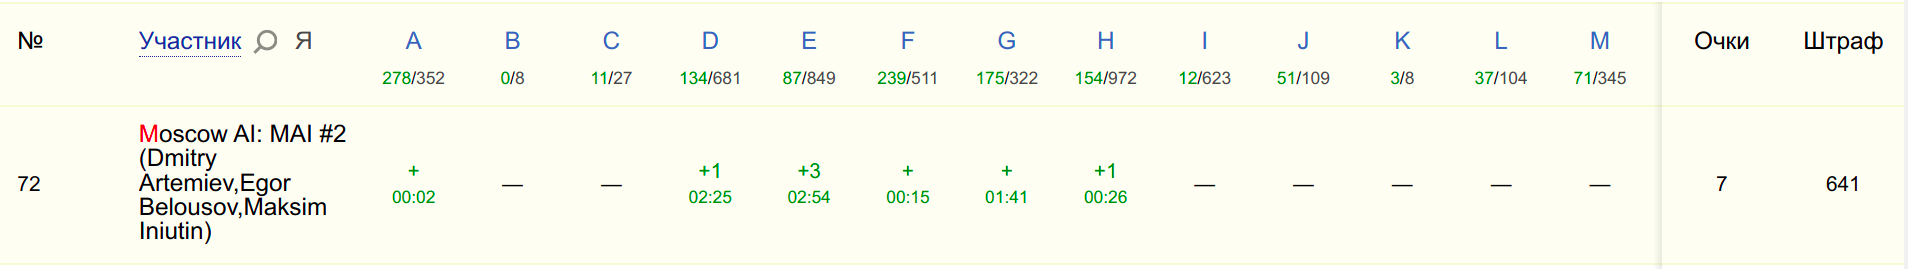
\includegraphics[width=\textwidth]{images/moscow_regional.png}\newline\noindent
\subsubsection*{Выводы}
Задача решена. Было 3 неудачных попытки.
\pagebreak

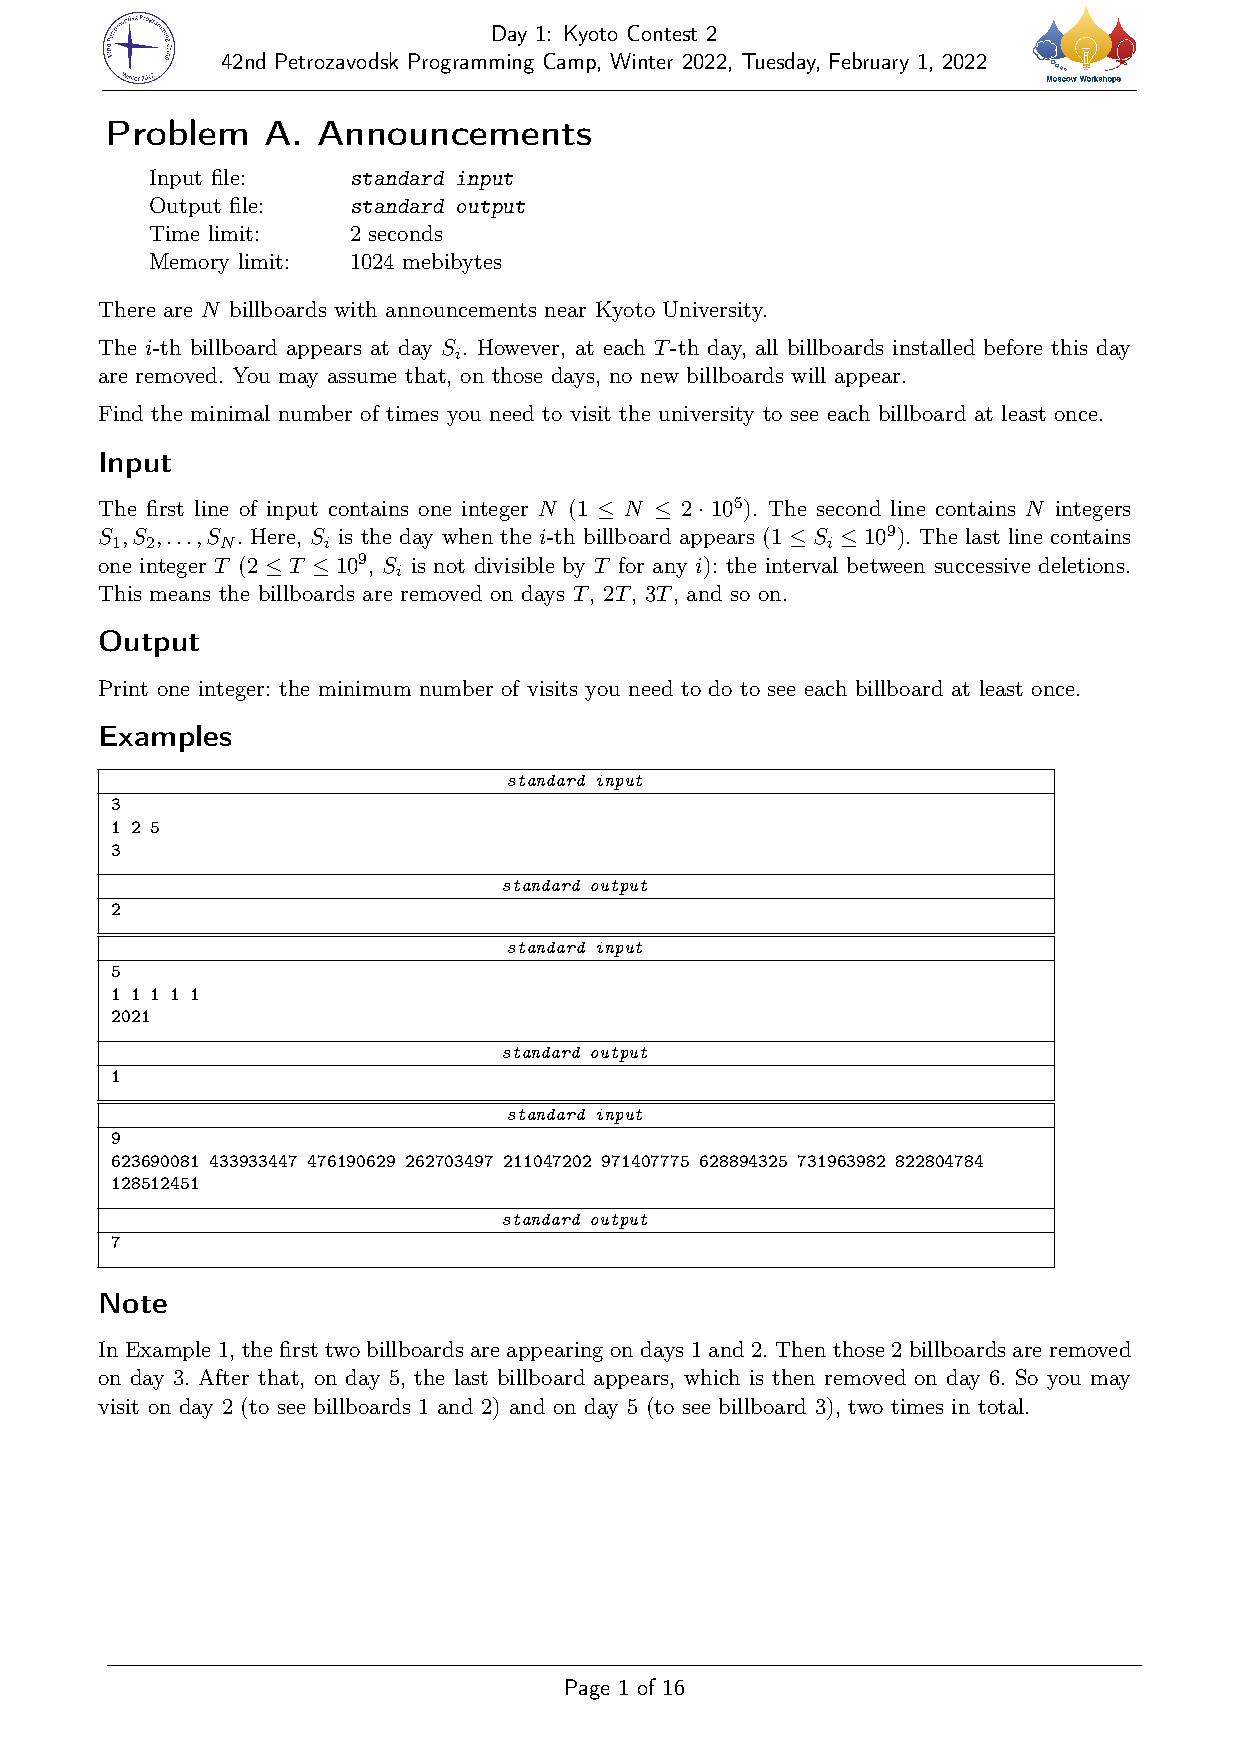
\includepdf[pages=1, scale=0.75, pagecommand=\subsection*{42nd Petrozavodsk Programming Camp, Winter 2022 Day 1}]{statements/220201/220201.en.pdf}
\subsubsection*{Идея решения}
Заметим, что все дни можно разделить на блоки по $T$ дней, тогда все биллборды в одном блоке мы можем посмотреть за один день, таким образом задача сводится к подсчету различных $\dfrac{a_{i}}{T}$ (округлив вниз). Это можно сделать отсортировав исходную последовательность, итоговая сложность $O(n \cdot \log{n})$.
\subsubsection*{Исходный код}
\lstinputlisting{src/220201.cpp}
\subsubsection*{Фрагмент турнирной таблицы}
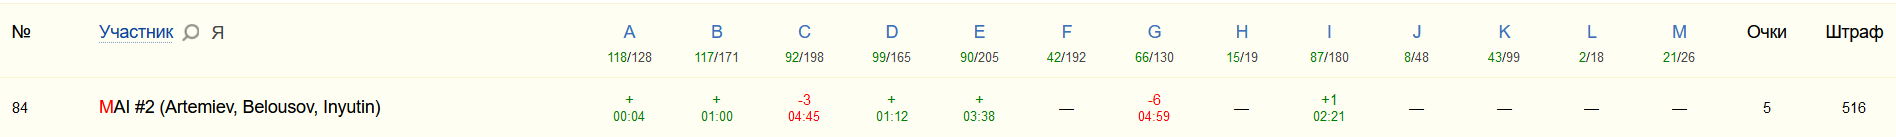
\includegraphics[width=\textwidth]{images/220201.png}\newline\noindent
\subsubsection*{Выводы}
Задача решена.
\pagebreak

\includepdf[pages=5, scale=0.75, pagecommand=\subsection*{42nd Petrozavodsk Programming Camp, Winter 2022 Day 2}]{statements/220202/220202.en.pdf}
\subsubsection*{Идея решения}
Будем решать немного обратную задачу: нужно набрать отрезков наибольшего веса, так чтобы они не образовывали компоненту размера более чем $K$. Отсортируем отрезки по левой границе. Тогда пусть $dp_{i}$ -- лучший ответ, если мы рассматриваем отрезки с $i$ по $n$, переберем количество отрезков и будем жадно с помощью $multiset$ оставлять самые дорогие. Итого решение работает за $O(n^2 \cdot \log{K})$
\subsubsection*{Исходный код}
\lstinputlisting{src/220202.cpp}
\subsubsection*{Фрагмент турнирной таблицы}
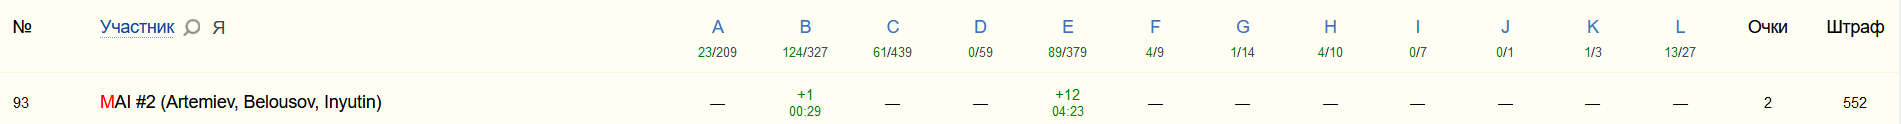
\includegraphics[width=\textwidth]{images/220202.png}\newline\noindent
\subsubsection*{Выводы}
Задача решена. Было 12 неудачных попыток.
\pagebreak

\includepdf[pages=6, scale=0.75, pagecommand=\subsection*{42nd Petrozavodsk Programming Camp, Winter 2022 Day 3}]{statements/220203/220203.en.pdf}
\subsubsection*{Идея решения}
Задачу можно легко свести к динамическому программированию на дереве. Все что нам требуется аккуратно обработать краевые случаи. Итоговая сложность $O(n)$.
\subsubsection*{Исходный код}
\lstinputlisting{src/220203.cpp}
\subsubsection*{Фрагмент турнирной таблицы}
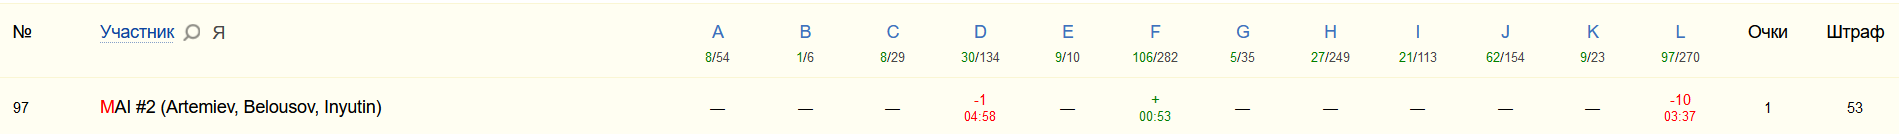
\includegraphics[width=\textwidth]{images/220203.png}\newline\noindent
\subsubsection*{Выводы}
Задача решена.
\pagebreak

\includepdf[pages=7, scale=0.75, pagecommand=\subsection*{42nd Petrozavodsk Programming Camp, Winter 2022 Day 4}]{statements/220204/220204.en.pdf}
\subsubsection*{Идея решения}
Ввиду небольших ограничений мы можем решить эту задачу по слоям с помощью динамического программирование на подмножествах. Будем считать лучший ответ для каждой маски и для каждого слоя. Переход делается за $O(4^m)$, итоговая сложность $O(n \cdot 4^m)$.
\subsubsection*{Исходный код}
\lstinputlisting{src/220204.cpp}
\subsubsection*{Фрагмент турнирной таблицы}
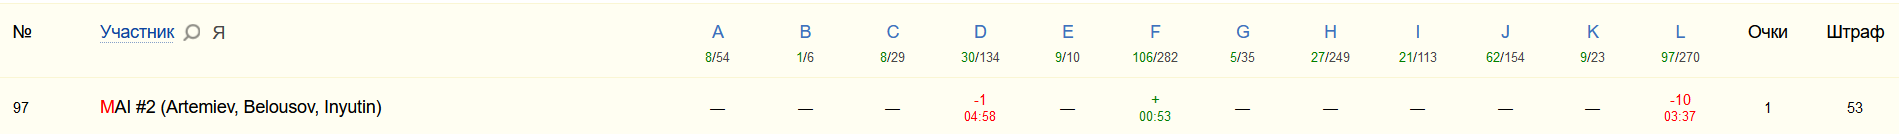
\includegraphics[width=\textwidth]{images/220203.png}\newline\noindent
\subsubsection*{Выводы}
Задача дорешена.
\pagebreak

\includepdf[pages=4, scale=0.75, pagecommand=\subsection*{42nd Petrozavodsk Programming Camp, Winter 2022 Day 5}]{statements/220206/220206.en.pdf}
\subsubsection*{Идея решения}
Сперва отсеим частные случаи: при $n = 1$ ответ $0$, а при $n = 2$ -- 1. В ином случае возьмем за корень не листовую вершину (такая гарантированно найдется), рассмотрим решение задачи для поддерева с корнем в $v$: для того, что бы все пути от листа к листу в поддереве были четными требуется, чтобы все пути от $v$ до листьев были одинаковой четности, тогда сделаем $dp[v][0]$ -- решения, если все пути четной длины, $dp[v][1]$ -- решение, если все пути нечетной длины. Переходы очевидны. Итоговая сложность $O(n)$.
\subsubsection*{Исходный код}
\lstinputlisting{src/220206.cpp}
\subsubsection*{Фрагмент турнирной таблицы}
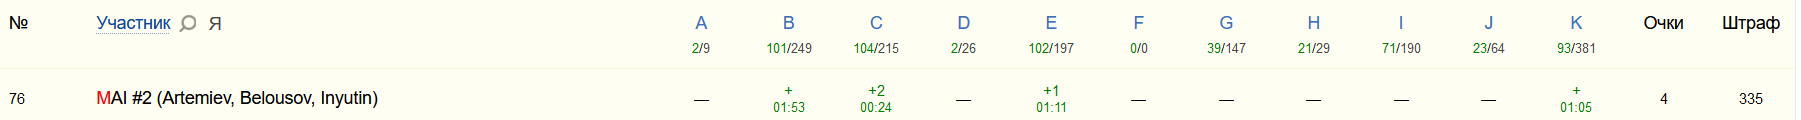
\includegraphics[width=\textwidth]{images/220206.png}\newline\noindent
\subsubsection*{Выводы}
Задача решена. Было 2 неудачных попытки.
\pagebreak

\includepdf[pages=13, scale=0.75, pagecommand=\subsection*{42nd Petrozavodsk Programming Camp, Winter 2022 Day 6}]{statements/220207/220207.en.pdf}
\subsubsection*{Идея решения}
Задача чисто комбинаторная, можно показать, что ответом является сумма чисел Стирлинга второго рода. Таким образом, задачу можно решить за $O((n + m)\log{C})$, где $C = 998244353$.
\subsubsection*{Исходный код}
\lstinputlisting{src/220207.cpp}
\subsubsection*{Фрагмент турнирной таблицы}
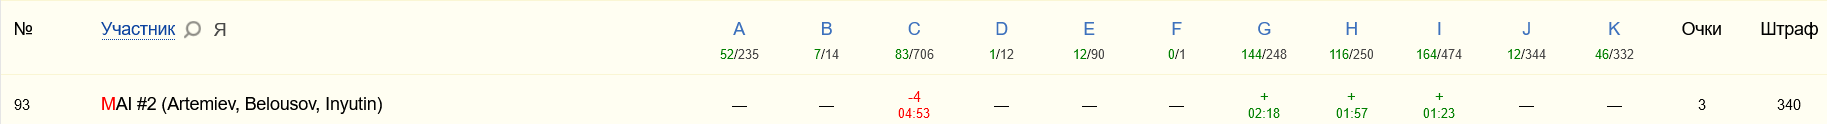
\includegraphics[width=\textwidth]{images/220207.png}\newline\noindent
\subsubsection*{Выводы}
Задача решена.
\pagebreak

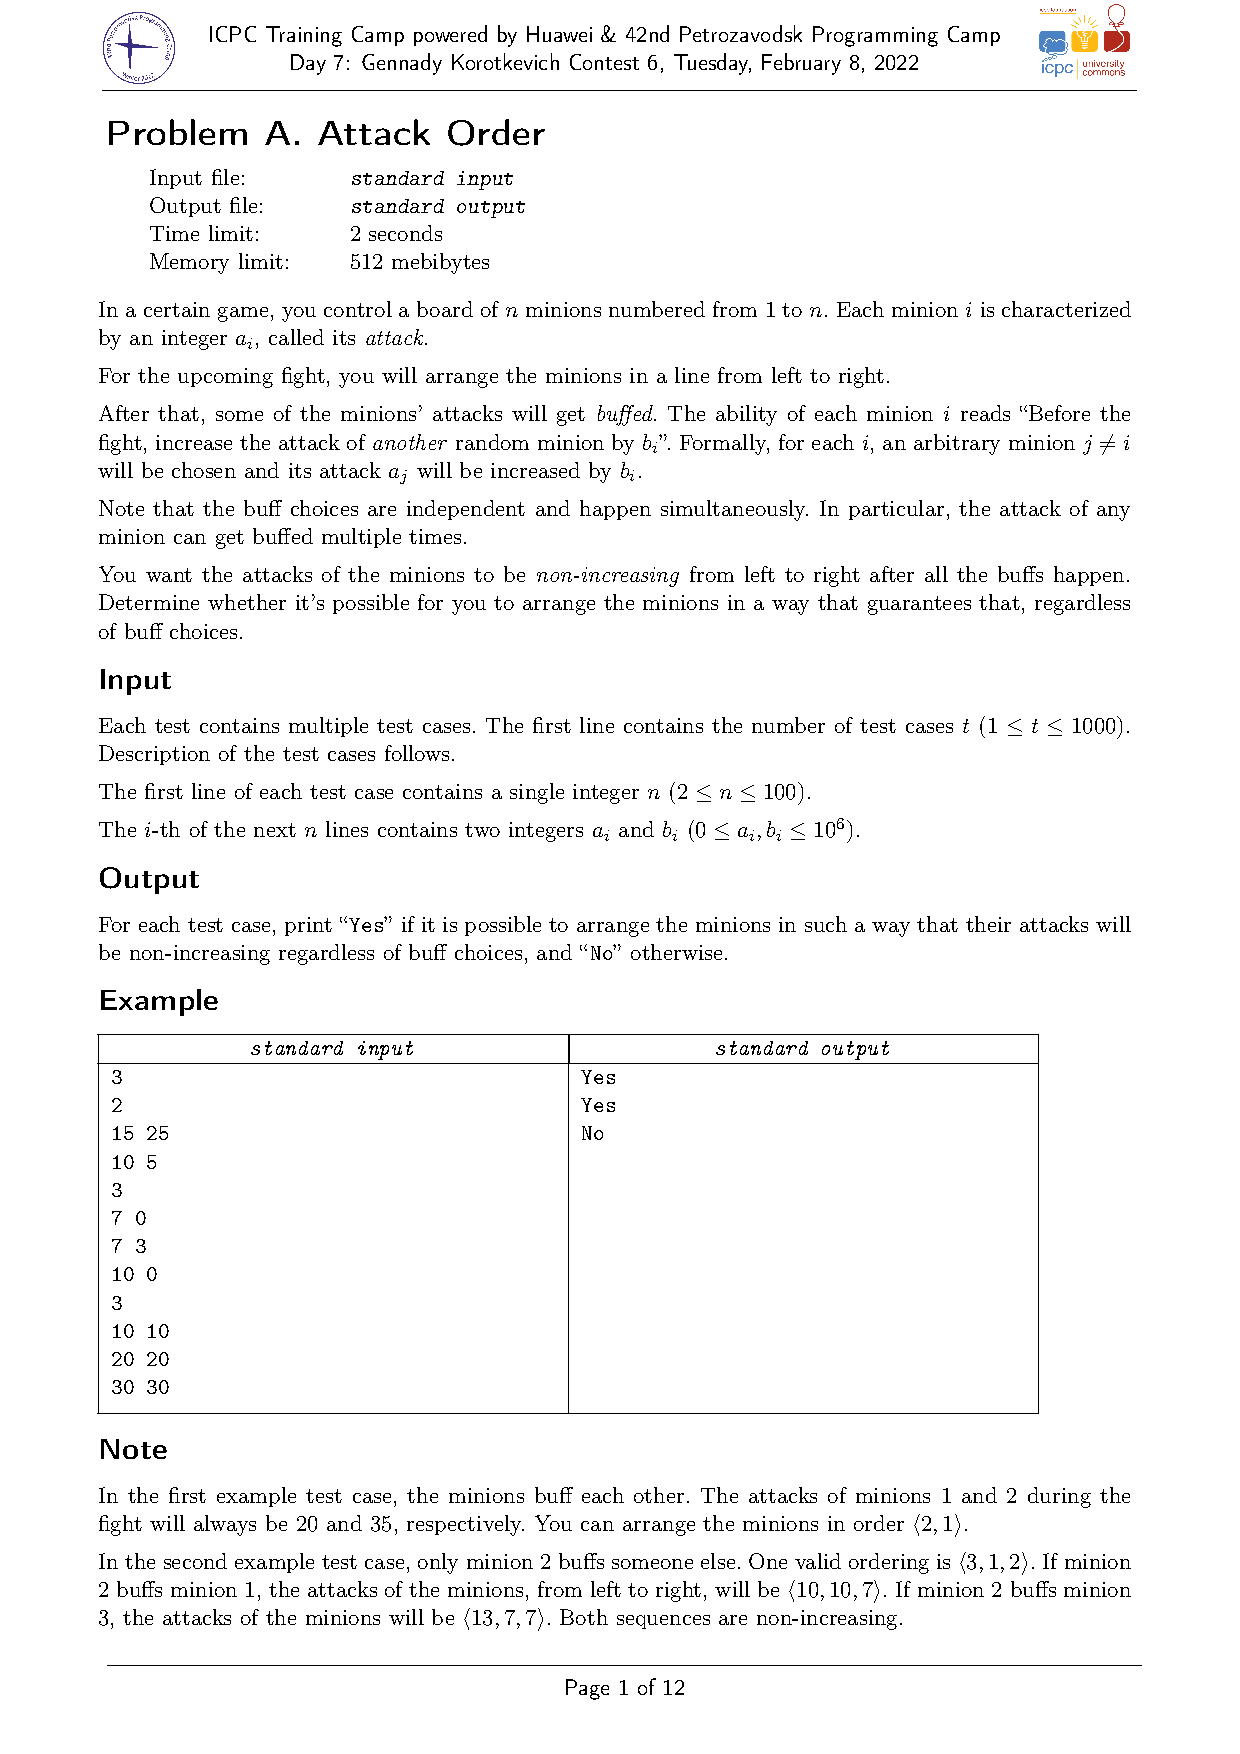
\includepdf[pages=1, scale=0.75, pagecommand=\subsection*{42nd Petrozavodsk Programming Camp, Winter 2022 Day 7}]{statements/220208/220208.en.pdf}
\subsubsection*{Идея решения}
Пусть $c_i$ -- это $a_i + \sum_{j != i} b_j$. Отсортируем изначальную последовательность по невозрастанию по $c_i$, в случае равенства сохраним относительный порядок. Теперь проверим для каждого элемента, что в худшем случае он все равно меньше, чем любой элемент перед ним. Итоговая сложность $O(n\cdot \log{n})$.
\subsubsection*{Исходный код}
\lstinputlisting{src/220208.cpp}
\subsubsection*{Фрагмент турнирной таблицы}
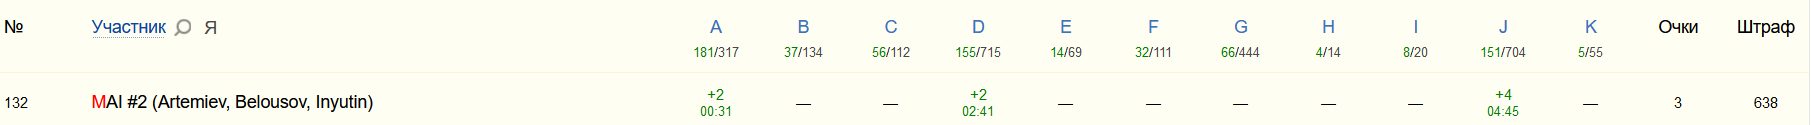
\includegraphics[width=\textwidth]{images/220208.png}\newline\noindent
\subsubsection*{Выводы}
Задача решена. Было 2 неудачных попытки.
\pagebreak

\includepdf[pages=16, scale=0.75, pagecommand=\subsection*{ICPC 2021-2022 NERC - Northern Eurasia Finals}]{statements/220413/220413.pdf}
\subsubsection*{Идея решения}
Будем последовательно рассматривать всех соседей из стартовой вершины. Запустим из очередного соседа поиск в глубину, но не будем заходить в начальную вершину, и пометим все вершины достижимые вершины, если в процессе поиска мы наткнулись на вершину, помеченную ранее, значит эта вершина может быть конечной вершиной $t$, остается только вывести 2 пути. Итоговая сложность $O(n)$.
\subsubsection*{Исходный код}
Сорвенование проходило очно, каждой команде предоставляли ноутбук. Исходный код недоступен.
\subsubsection*{Фрагмент турнирной таблицы}
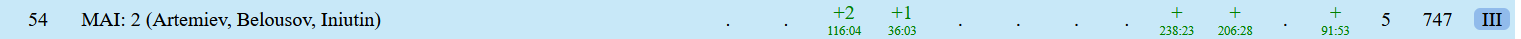
\includegraphics[width=\textwidth]{images/220413.png}\newline\noindent
\subsubsection*{Выводы}
Задача решена.
\pagebreak

\includepdf[pages=7, scale=0.75, pagecommand=\subsection*{Prefinals Moscow Workshop 2022 Day 1}]{statements/220418/220418.en.pdf}
\includepdf[pages=8, scale=0.75, pagecommand=\subsection*{Prefinals Moscow Workshop 2022 Day 1}]{statements/220418/220418.en.pdf}
\subsubsection*{Идея решения}
Заметим, что циклы do-while можно представить в виде скобочной последовательности. Заменим все if-goto на do-while в соответствии с правилами. Теперь заменим do на открывающую скобку, а while на закрывающую. Проверим, является ли эта последовательность ПСП. Это и будет нашим ответом. Сложность для сортировки всех строк программы $O(n \cdot \log{n})$ и сложность проверки на ПСП $O(n)$, поэтому асимптотика $O(n \cdot \log{n})$.
\subsubsection*{Исходный код}
\lstinputlisting{src/220418.cpp}
\subsubsection*{Фрагмент турнирной таблицы}
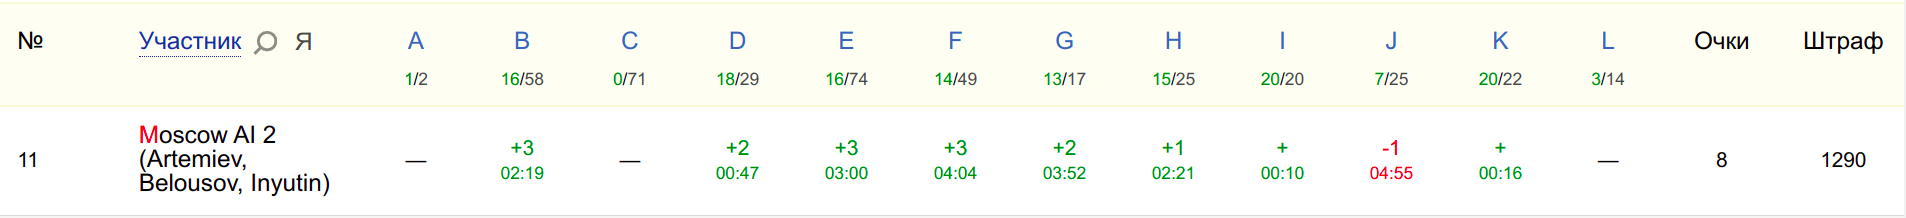
\includegraphics[width=\textwidth]{images/220418.png}\newline\noindent
\subsubsection*{Выводы}
Задача решена. Было 2 неудачных попытки. Изначальная идея решения задачи была неверна.
\pagebreak

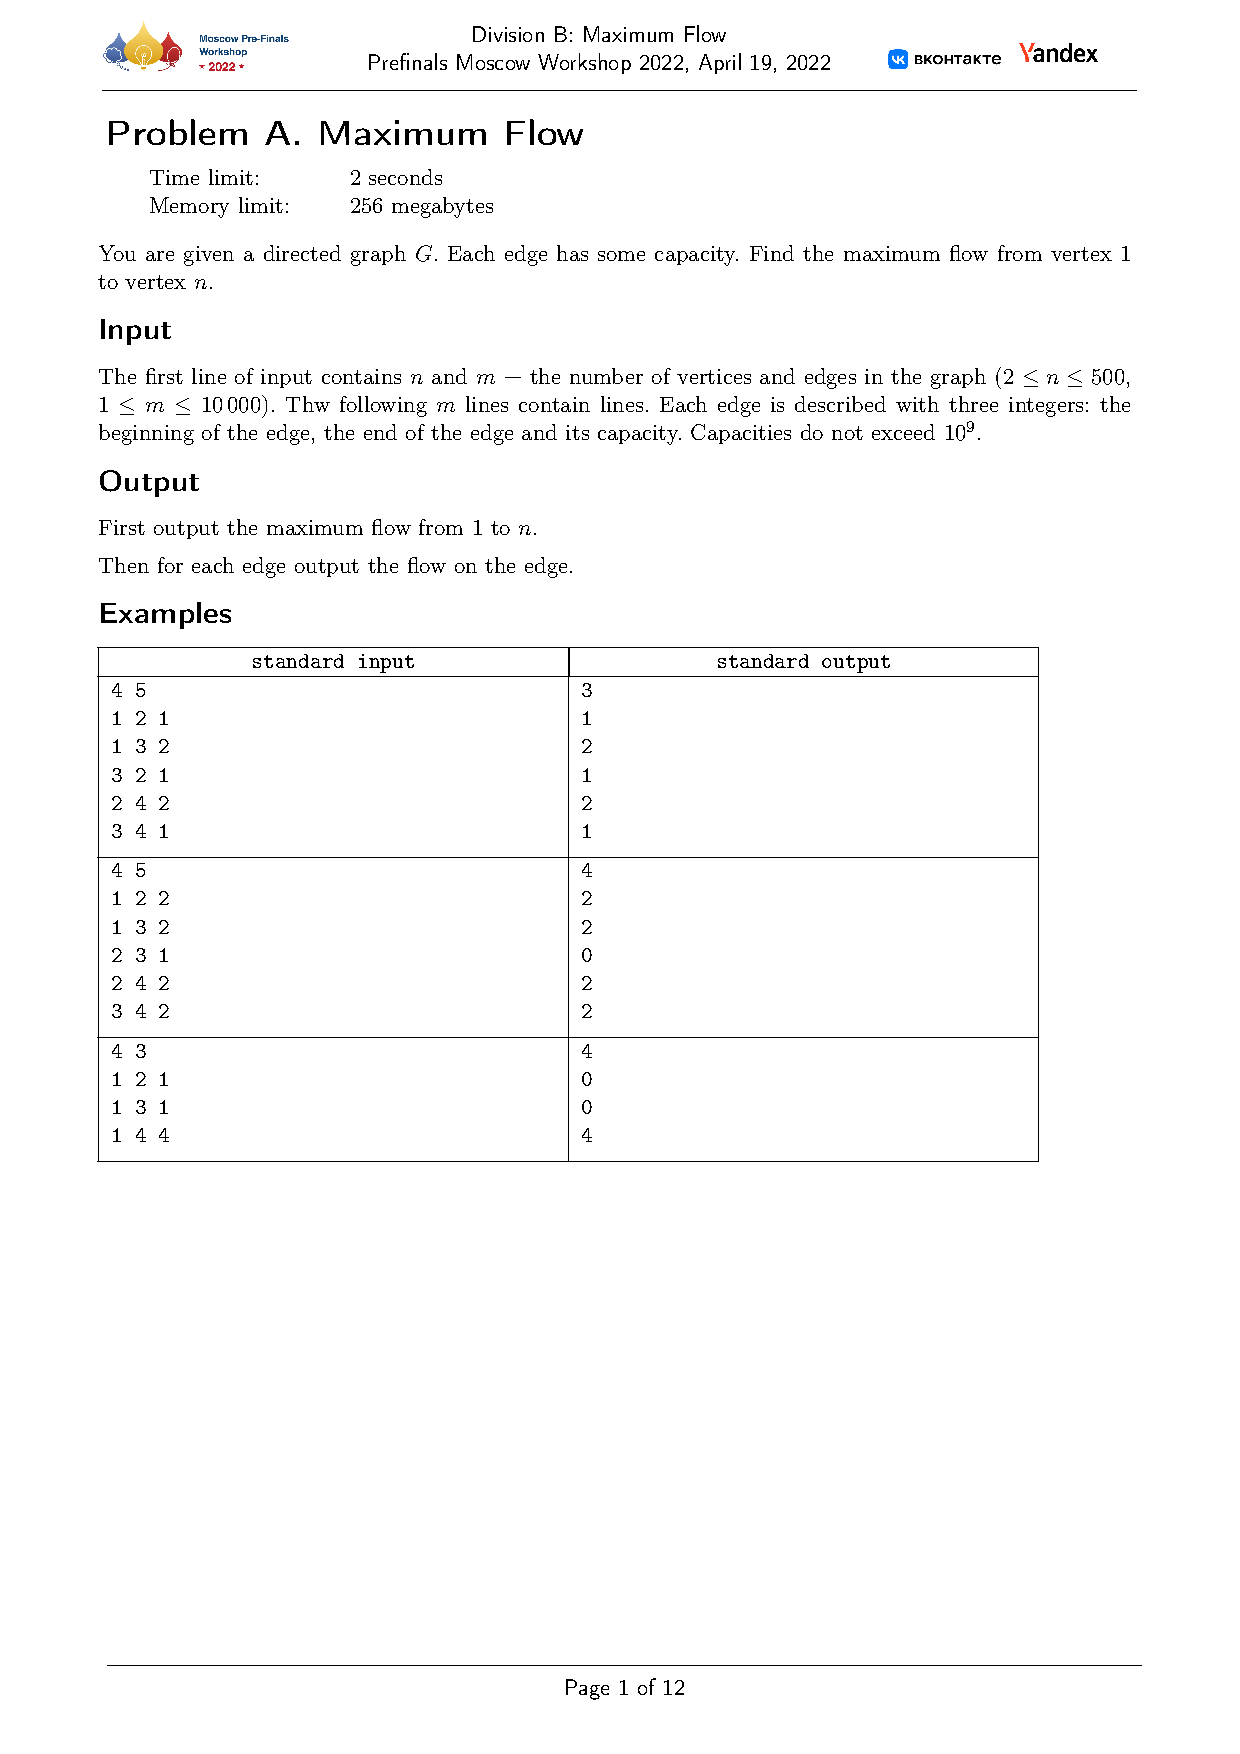
\includepdf[pages=1, scale=0.75, pagecommand=\subsection*{Prefinals Moscow Workshop 2022 Day 2 Div B}]{statements/220419/220419b.en.pdf}
\subsubsection*{Идея решения}
Это классическая задача на поиск максимального потока в транспортной сети. Алогритм Диница имеет сложность $O(n ^ 2 \cdot m)$, что вполне удовлетворяет заданным ограничениям. Применение масштабирования улучшает сложность до $O(n \cdot m \cdot \log{C_{max}})$, где $C_{max}$ --- максимальная величина пропускной способности в транспортной сети.
\subsubsection*{Исходный код}
\lstinputlisting{src/220419.cpp}
\subsubsection*{Фрагмент турнирной таблицы}
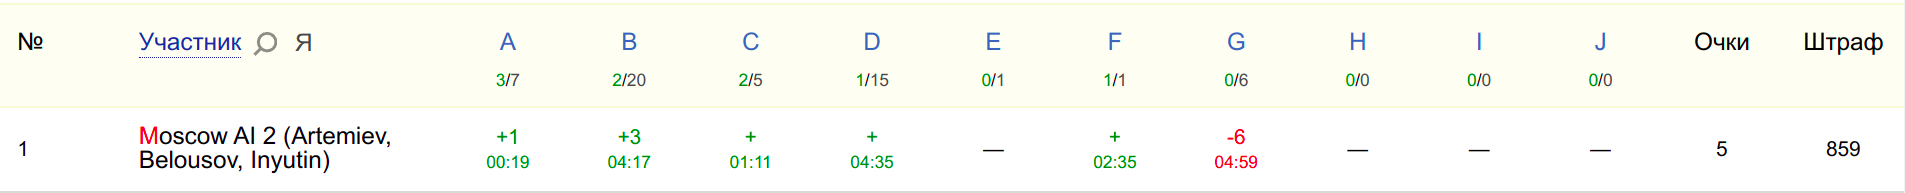
\includegraphics[width=\textwidth]{images/220419.png}\newline\noindent
\subsubsection*{Выводы}
Задача решена. Была 1 неудачная попытка.
\pagebreak

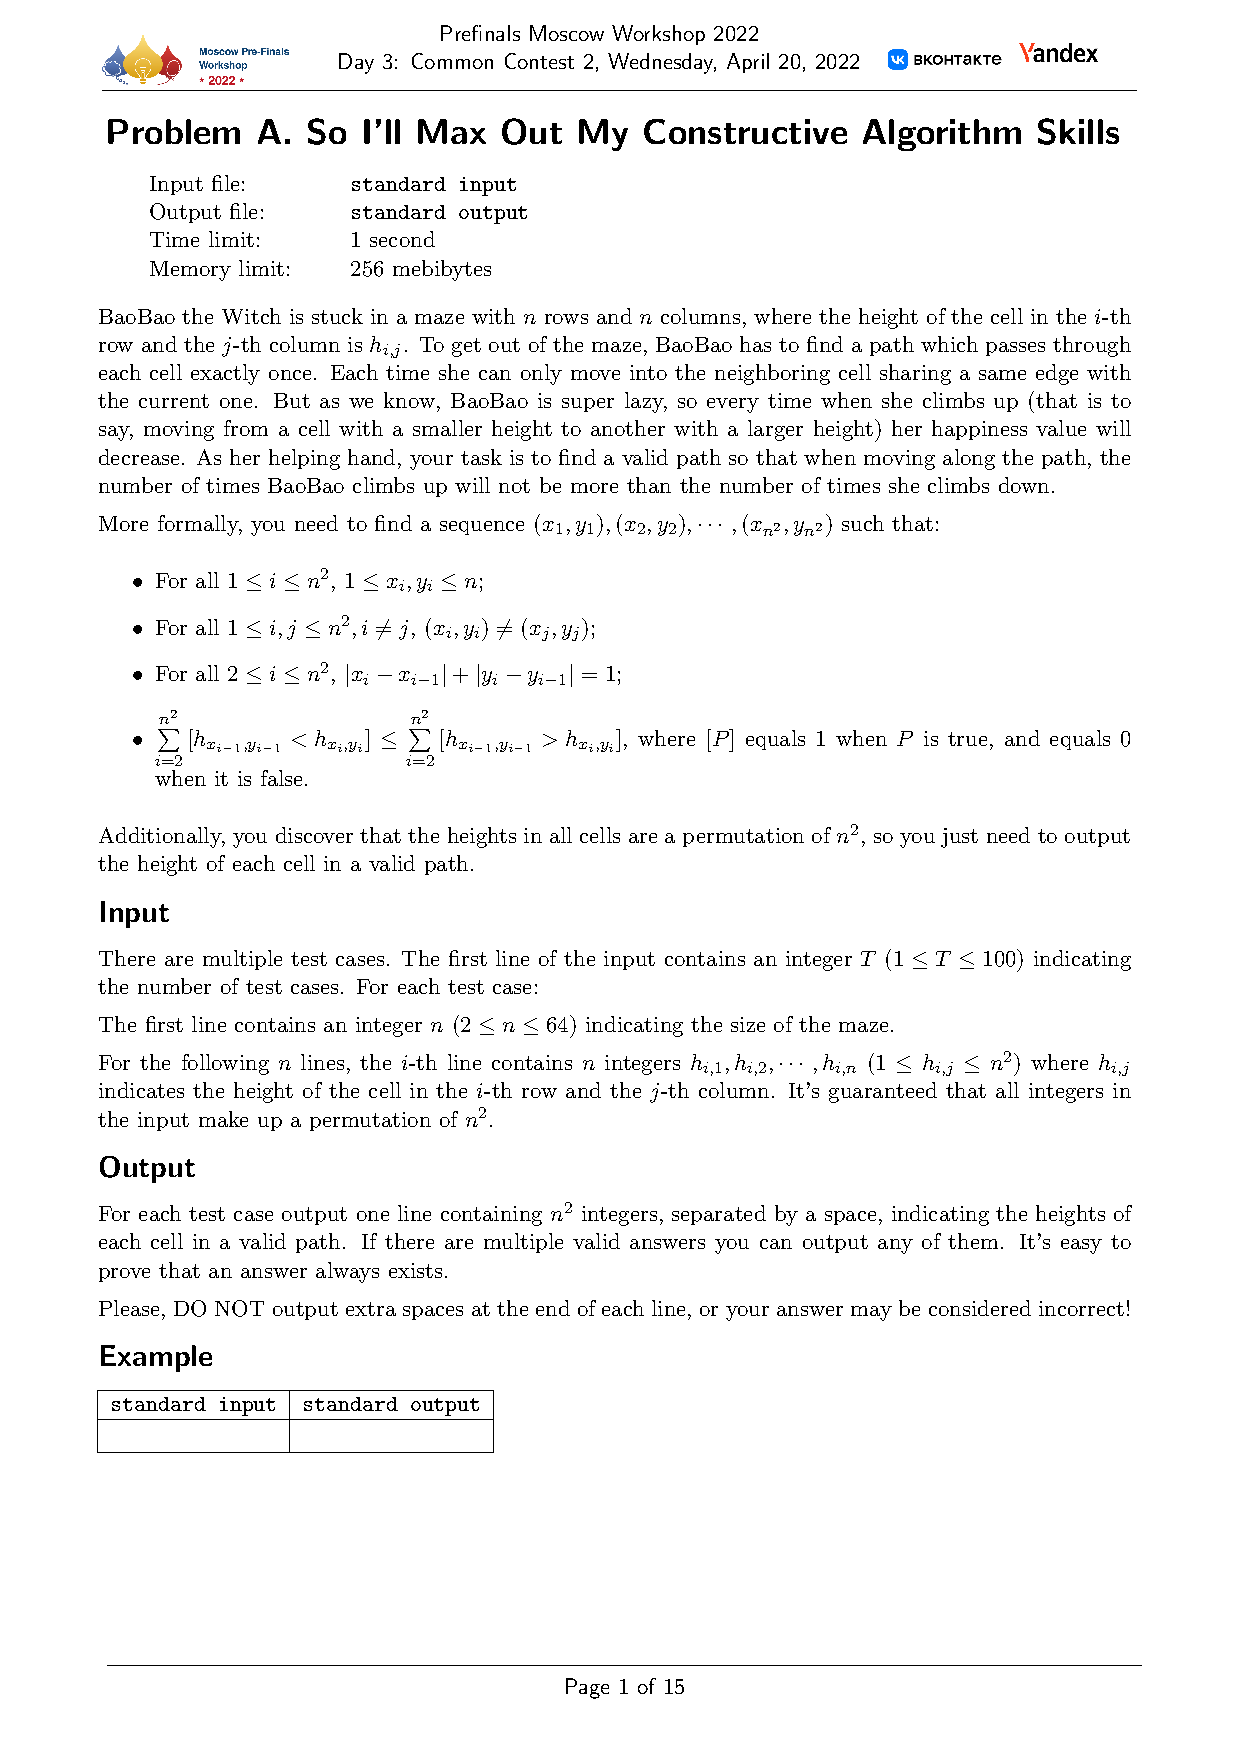
\includepdf[pages=1, scale=0.75, pagecommand=\subsection*{Prefinals Moscow Workshop 2022 Day 3}]{statements/220420/220419.en.pdf}
\subsubsection*{Идея решения}
Пройдём по всему полю змейкой, начиная с левого верхнего угла. Проверим, является ли этот путь хорошим. Если это так, то ответ найден. В противном случае ответ --- это наш путь в обратном порядке, так как теперь вместо подъёмов будут спуски, а вместо спусков подъёмы. Сложность $O(T \cdot n ^ 2)$.
\subsubsection*{Исходный код}
\lstinputlisting{src/220420.cpp}
\subsubsection*{Фрагмент турнирной таблицы}
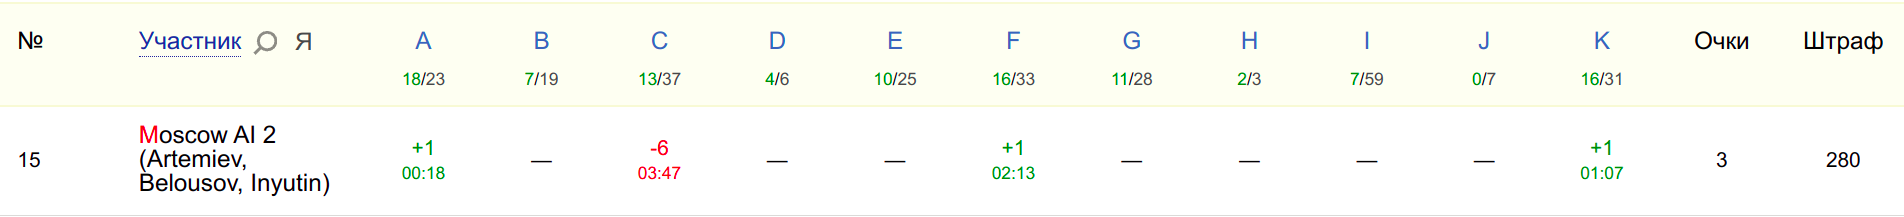
\includegraphics[width=\textwidth]{images/220420.png}\newline\noindent
\subsubsection*{Выводы}
Задача решена. Была 1 неудачная попытка.
\pagebreak

\includepdf[pages=9, scale=0.75, pagecommand=\subsection*{Prefinals Moscow Workshop 2022 Day 4 Div B}]{statements/220422/220422b.pdf}
\subsubsection*{Идея решения}
Требуется реализовать алгоритм Укконена построения суффиксного дерева за линейное время.

Алгоритм Укконена в самой простоей реализации имеет сложность $O(n^3)$, так как добавляет каждый суффикс каждого префикса строки в отличии от добавления всех суффиксов строки. Основная идея в том, чтобы оптимизировать его и получить сложность $O(n)$.

Заметим, что проще будет продлевать суффиксы на один символ. В некоторых случаях при продлении можно идти не по всем символам, а сразу по ребру дерева, что значительно уменьшает число шагов.

Пусть в суффиксном дереве есть строка $x\alpha$ ($x$ --- первый символ строки, $\alpha$ --- оставшаяся строка), тогда $\alpha$ тоже будет в суффиксном дереве, потому что $\alpha$ является суффиксом $x\alpha$. Если для строки $x\alpha$ существует некоторая вершина $u$, то существует и вершина $u$ для $\alpha$. Ссылка из $u$ в $v$ называется суффиксной ссылкой.

Суффиксные ссылки позволяют не проходить каждый раз по дереву из корня. Для построения суффиксных ссылок достаточно хранить номер последней созданной вершины при продлении. Если на этой же фазе мы создаём ещё одну новую вершину, то нужно построить суффиксную ссылку из предыдущей в текущую.

Сложность алгоритма с использованием продления суффиксов и суффиксных ссылок $O(n^2)$.

Для ускорения до $O(n)$ нужно уменьшить объём потребляемой памяти. Будем в каждом ребре дерева хранить не подстроку, а только индекс начала и конца подстроки.

У исходной строки $n$ суффиксов и будет создано не более $n$ внутренних вершин, в среднем продление суффиксов работает за $O(1)$.

При использовании всех вышеописанных эвристик получим временную и пространственную сложность $O(n)$.
\subsubsection*{Исходный код}
\lstinputlisting{src/220422.cpp}
\subsubsection*{Фрагмент турнирной таблицы}
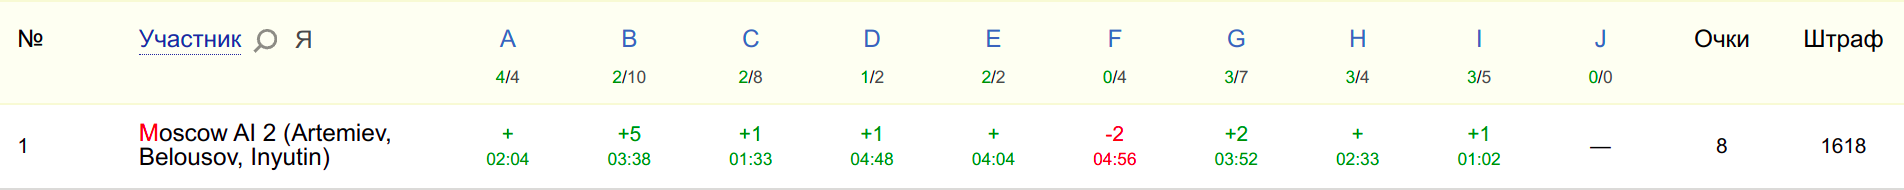
\includegraphics[width=\textwidth]{images/220422.png}\newline\noindent
\subsubsection*{Выводы}
Задача решена. Была 1 неудачная попытка. Забыли учесть знак числа.
\pagebreak

\includepdf[pages=8, scale=0.75, pagecommand=\subsection*{Prefinals Moscow Workshop 2022 Day 5 Div B}]{statements/220423/220423b.en.pdf}
\subsubsection*{Идея решения}
Пусть $a = 7310$ и $b = 2468$. Можно записать $a = 7 \cdot 10 ^ 3 + 3 \cdot 10 ^ 2 + 1 \cdot 10 + 0$ и $b = 2 \cdot 10 ^ 3 + 4 \cdot 10 ^ 2 + 6 \cdot 10 + 8$.

Пусть $A(x) = 0 + 1 \cdot x + 3 \cdot x ^ 2 + 7 \cdot x ^ 3$ и $B(x) = 8 + 6 \cdot x + 4 \cdot x ^ 2 + 2 \cdot x ^ 3$. Тогда $A(10) = a$ и $B(10) = b$. Если мы вычислим ДПФ для многочленов $A(x)$ и $B(x)$, то перемножив их значения ДПФ в одних и тех же точках, мы получим значения ДПФ для $(A \cdot B) (x)$, то есть
$$DFT(A \cdot B) = DFT(A) \cdot DFT(B)$$

Применив обратное преобразование Фурье к полученному и вектору, мы получим коэффициенты многочлена $(A \cdot B) (x)$. Так мы смогли перемножить два многочлена, используя БПФ:
$$ (A \cdot B) (x) = InverseDFT(DFT(A \cdot B)) = InverseDFT(DFT(A) \cdot DFT(B)) $$

Так как $A$ и $B$ изначально представляли числа $a$ и $b$, выполним перенос разрядов, чтобы получить многочлен, предсталвяющий $a \cdot b$.

Такой подход позволяет перемножать два многочлена за $O(n \cdot \log(n))$. Мы смогли представить два числа в виде многочленов, таким образом смогли перемножить два числа за такую же асимптотику $O(n \cdot \log(n))$.
\subsubsection*{Исходный код}
\lstinputlisting{src/220423.cpp}
\subsubsection*{Фрагмент турнирной таблицы}
\includegraphics[width=\textwidth]{images/220423.png}\newline\noindent
\subsubsection*{Выводы}
Задача решена. Была 1 неудачная попытка. Забыли учесть знак числа.
\pagebreak

\includepdf[pages=9, scale=0.75, pagecommand=\subsection*{RuCode 5.0 Championship, Division A-B}]{statements/220424/ab-ru.pdf}
\subsubsection*{Идея решения}
Механизм критического выстрела описывается распределением Бернулли с известными формулами. Посчитаем минимальное вероятность $p$ такую, что вероятность успеха из $k$ опытов была бы минимум $b$. Для этого перебирём все возможные вероятности и выведем первую подходящую. Сложность $O(100 \cdot t \cdot k)$.
\subsubsection*{Исходный код}
\lstinputlisting{src/220424.cpp}
\subsubsection*{Фрагмент турнирной таблицы}
\includegraphics[width=\textwidth]{images/220424.png}\newline\noindent
\subsubsection*{Выводы}
Задача решена. Было 2 неудачных попытки. Пришлось переписать решение на Python, так как точности типа double не хватило.
\pagebreak
